\documentclass[11pt]{article}
%\usepackage[round]{natbib}
\graphicspath{./plots/}
\usepackage{amsfonts}
\usepackage{amsmath}
\usepackage{paralist}
\usepackage{subfig}
\usepackage{times}
\usepackage{latexsym}
\usepackage{graphicx}
\usepackage[T1]{fontenc}
\usepackage{tikz}
\usepackage{url}
\usepackage{pgfplotstable}
\usepackage{titlesec}
\usepackage{color}
\usepackage{lipsum,adjustbox}
\usepackage[font={small}]{caption}
\usetikzlibrary{positioning}

\usepackage{acl2017}


\begin{document}
	
	\title{Improved Statistical Evaluation for Grammatical Error Correction}
	
	\author{
		Leshem Choshen\textsuperscript{1} and Omri Abend\textsuperscript{2} \\
		\textsuperscript{1}School of Computer Science and Engineering, \textsuperscript{2} Department of Cognitive Sciences \\
		The Hebrew University of Jerusalem \\
		\texttt{leshem.choshen@mail.huji.ac.il, oabend@cs.huji.ac.il}\\
	}
	
	
	\maketitle
\begin{abstract}
	xxx
	
\end{abstract}

\section{Main ideas(abstract base)}

We propose two notions of conservatism:semantic conservatism and formal
conservatism and state the former one is mostly the one we strive
for when correcting.

We state semantic annotation is valuable for error correction and
error assessment.

We present a new methods to compare UCCA annotation

we show UCCA can be used for annotating ungrammatical texts

we show UCCA is stable over grammar correction,
 and hence the semantics it captures is surely stable too.

we show state of the art error correction methods are highly formally
conservative (why formal and not structural or another name?)

We show current correction methods are too formally conservative,
they don't change enough sentence boundaries, enough words and enough
characters.

We suggest one of the factors contributing to over formal conservatism
is having only a small number of references covering low percentage
of the possible correction. It affects both assessment and development.
In the development process we would expect good learning to understand
not to try to correct complicated sentences as those will be very
likely to be judged a mistake. Even when they are not.

Current correctors undercorrect, maybe due to lack of gold references.

Current assessment is a an under assessment giving a much lower score
than ought to be. What affects it is mainly the number of annotations for each sentence in the gold standard.

We give confidence intervals for current state of the art and predict how their length will change. 
We emphasize that lowering confidence interval length is a balancing problem, 
because variance is dependent on the number of sentences and the number of corrections per sentence.


\section{Opening}

In the history of error correction, conservatism was considered an
important trait of an error correcting system\cite{brockett2006correcting}.
This was also the reason why $F_{0.5}$ became since conll2014\cite{ng2014conll}
the measure of choice for error correction evaluation, emphasizing
precision over recall. This emphasis can be understood as encouraging
avoidance of wrong corrections at the cost of correcting less errors
overall. The thought that stands behind such emphasis is that a user
would be understanding towards errors he did, of which he is probably
not even aware, not being corrected, but would not be so understanding
when he sees a correction changes what he knows to be correct. We want to refine
this idea and suggest that there are subtleties we better address
in this intuition.

There are two different conservatism
types, semantic conservatism and formal one, of which the semantic
is the one we strongly need to adopt and the formal is merely a technicality
for the user. in part 1{*}{*}make sure it is right where all is written,
cross references{*}{*}we address the two conservatism types in part
2 we show semantics can be a consistent and measurable allowing use
of it for ensuring semantic conservatism in part 3 we show current
systems tend to be too conservative when compared with human
corrections in part 4 we suggest this to be an outcome of the evaluation
measure used, being formally conservative and lacking. We further develop
 the discussion about the statistics of corrections 
 and about evaluation significance and value. 
 An analysis that is a basis for understanding this formal conservatism, 
 but also necessary by itself.

\section{Conservatism - not a single concept}

\subsection{what we really wish to be conservative about}

In the task of grammatical error correction it is important to be
conservative, not to overcorrect. The user expects the minimum corrections
necessary and wants no intervention in what he wishes to say. More
specifically, he expects that what he has said would not be changed
into something he did not. In this we may find two notions of conservatism,
formal conservatism and semantic conservatism. Where any change in
the original string would not be considered formal conservative, only
changes in meaning are accounted for invalidating semantic conservatism. 

In many of the uses for correction,
the user does understand his grammar is not perfect and would accept
a change in grammar when needed. Because of this approval we also
hypothesis, and it may call for a user study to prove or disprove
this hypothesis, that users might accept a correct text unit of theirs
being corrected to another correct text unit with the same meaning.
This would be an example of being semantically conservative but not formally so.
Maybe even more importantly, we aim to have as many correct sentences
as possible, but as the grammar isn't fully correct in the first place,
nor is the user's understanding of it, failing to correct grammar
is acceptable. Changing meaning will be totally unacceptable, and
also surely detectable by the user. In other words, the users do expect
the corrector to be active and not too formally conservative, but
only as long as it is semantically conservative. 

Moreover, as corrections are based on statistics, they might even
just correct to a more common way of saying the same thing. Such unnecessary
correction is not formally conservative, and at grammatical error
correction maybe be unwanted, but not strictly unwanted as overall
it is semantically conservative still. Additionally, some may even
say this correction is a needed one because it has a better grammar considering
Fuzzy Grammar\cite{lakoff1973fuzzy,madnani2011they} or a more fluent
way to say the exact same thing. The latter was suggested as a necessary
shift in the goals of error correction\cite{sakaguchi2016reassessing}.
Considering all this, we propose that next generation grammatical
error correctors and evaluation will be focused on semantic conservatism
when possible rather than on formal conservatism.

\section{Semantics in learner language}

\subsection{Uses of semantic annotation}

As semantic annotation was not used before to aid grammatical error
correction, it is worth mentioning the a-priori reasons for developing
it. The first and perhaps the most obvious use of semantic annotation
would be to use it as a feature for correctors. The annotation may
capture the gist that is supposed to stay the same when correcting,
allowing the corrector to filter results or re-rank them based on
the annotation or just to put it inside the mesh of features and learn
automatically what to do with it, just as done with grammatical annotation.
Later in this section we will not only discuss how to compare those
features, specifically UCCA, but also why it is suspected to be a
valuable feature.

Another approach of using semantic annotation would be for assessment.
Reliable assessment by a gold standard might be hard to obtain (see
\ref{sec:May-lack-of}), and human annotation for each output is great\cite{madnani2011they}
but costly, especially considering development process. In these conditions,
given a reliable semantic annotation we can enhance the reliability
of our assessment. One way to do that might be to decouple the meaning
from the structure. We propose a broad idea for a reduction from grammatical
error detection and a comparable semantics annotation to grammatical
error correction assessment. Lets assume we have both a reliable error
detection tool and a good way to measure semantic changes. Then, we
can transform assessment to a 3 steps assessment. First, detect errors
in the original text. Assess the percentage of needed corrections
that were actually corrected. Second, assess how much of was the semantics
changed. Give a negative score for changing semantics. Third, use
the error detection again to assess how many errors exist in the correction
output, whether uncorrected by the corrector or new errors presented
by the correction process itself. \\

This assessment was partially inspired by the WAS evaluation scheme\cite{chodorow2012problems},
in short it states we should account in the assessment for 5 types,
not only the True\textbackslash{}False Positive\textbackslash{}Negative
but also for the case where the annotation calls for a correction,
and the system did a correction, but one that is unlike the annotation's
one. With the proposed assessment we can measure how many of the corrections
were corrected correctly (First + Second), and how many errors do
we have eventually (Third) and combine them to get something similar
to the Precision Recall that is widely used. We can also account for
the places where the error was detected and check if it was corrected
in a way that makes it grammatical and did not change semantics, the
fifth type. We do that without getting a human to confirm this is
indeed a correction.

This system would be even more informative than the current one. Allowing assessment of
what exactly is the part in which a corrector failed. Answering questions
like: was it over formally conservative and did not make enough corrections?
Was it making changes in the right places but not correcting grammar
successfully? Was the system correcting grammar but changing things
it was not supposed to? etc.

\subsection{grammar can be annotated but is ill defined}

Syntactic representation is very popular and useful in many NLP tasks{*}{*}cites{*}{*}.
Thus, one thought that rises to mind is to use grammar annotation
to evaluate corrections. While not useless, this approach is not well
defined, and unclear bot practically and theoretically. One might
say that the grammar would be the one induced by the actual words
that appear in the sentence. This would lead to annotation that calls
for applying the syntax of Proper English to the different learner
languages that just don't correspond to it. Thus, the structures may
differ between different learners and they will tell us little about
how to understand the sentence. This approach was being pursued in
\cite{berzak2016universal}. 

Others may suggest, and indeed they have\cite{nagataphrase}, an opposite
approach, saying the grammar meant by the learner is the one we should
tag, but that requires having a corrected form of the sentences. Later\ref{sec:May-lack-of}
we show that for many sentences different corrections are possible.
And where as sentences differ so does their grammar. later in this
section, we propose semantic annotation as a well defined structure.

\subsection{Learner language can be annotated by UCCA}

At least theoretically, semantics are well defined even on ungrammatical
text. With the right tools we might capture at least some of the semantics
of sentences and use them for whatever we wanted grammar for and for
other tasks. In this work we will use Universal Conceptual Cognitive
Annotation (UCCA)\cite{abend2013universal}, we will show that practically
there are semantic annotation schemes that can be used for the purposes
discussed.

But as in the syntactic representation, before we can claim anything
about semantics using UCCA it is needed to show that UCCA is even
consistent when applied to ungrammatical language such as learner
language. To do that we used NUS\cite{dahlmeier2013building} a parallel
corpus of learner language and corrected versions which is the de
facto standard since CoNLL 2013\textbackslash{}14 shared tasks \cite{kao2013conll,ng2014conll}.
The NUS corpus consists of paragraphs of about 400 words each about
various topics. We employed two cognition graduate students, both
with background of working for a couple of years as translator. Each
one had received the guidelines to read and annotated a couple of
proper English paragraphs and then learner language paragraphs as
an exercise. These paragraphs were compared between the annotators
and each disagreement discussed in the hope of finding common annotation
mistakes and choosing a methodological approach to borderline cases.
After that each annotator has annotated 2 learner language paragraphs
consisting of almost 800 UCCA nodes each. Over the uncoordinated paragraphs
we computed the strict inter annotator agreement mentioned by \cite{abend2013universal}
considering each Node in the directed acyclic graph (DAG) of UCCA
annotation as agrees if and only if its label and the labels of all
its span leaves were considered to have the same labels respectively,
from that we derive an F1 score. 

We got an F1 score for the inter annotator agreement of 0.845 with
Precision 0.834 and Recall 0.857 we see that as enough to be a proof
that UCCA can be applied to, especially considering those numbers
are a bit higher than the inter annotator agreement reported in the
reported originally for formal English\cite{abend2013universal}.
We explain the rise in agreement by the fact that the guidelines and
procedures were refined since UCCA was first introduced and not to
superiority of UCCA for annotating learner language. A similar F1
score for inter annotator agreement (0.849) over 2 corrected paragraphs
suggests the same.

\subsection{Semantics are preserved when correcting grammar}

As a next step each annotator annotated corrected paragraphs corresponding
to ones he already annotated, 7 different paragraphs were annotated
in this way. To avoid misleading high score due to the fact that each
annotator annotated both the learner language paragraph and the corrected
paragraph 3 different tuples of paragraphs were annotated by both
annotators allowing a cross comparison, meaning that for each paragraph
we compared the annotation of the learner language done by one annotator
with the annotation of the other annotator done for the corrected
paragraph and vice versa. 

As a next step a comparison between the annotations was needed, but
there exists no measure for how similar two different UCCA annotations
of different texts are. We considered using suggested semantic measures
such as SMATCH\cite{cai2013smatch}but it can not work for UCCA or
DAG similarity measures such as graph kernels (e.g.\cite{kashima2003marginalized}),
but those tend to work on bigger graphs and would be the wrong tool
for the small UCCA DAGs. Thus, a new measure is called upon.

\subsection{Similarity measures\label{subsec:Similarity-measures}}

We propose several new methods to compare UCCA annotation of a learner\\
language with UCCA annotation of corrected texts, giving a more accurate
measure than the upper bound suggested by \cite{sulem2015conceptual}for
comparing two parallel texts in different languages, while keeping
the essence of comparing how many of the aligned nodes conserve meaning
and tag. For that we may think for a moment on error correction as
translation from learner language to Proper English, and a good translation
would be a translation which keeps the meaning but has the syntax
of English. Considering that, just like in translation we can align
words from the learner language to the corresponding words in English
and keep record of how many of those nodes kept their labels.

As comparing labels is trivial, and done before us. We should focus on how we propose to
align nodes. First, note that alignment should not be at
the token level, as we want to allow tokens to be corrected - replaced or removed -
as long as the higher structures convey the same meaning. We thus
prune the labels above the leaves, the tokens of the sentence. To
define an alignment of the nodes, we suggest some possible ways, all
based on first aligning the words in order to give order to the DAG
and then comparing the structure in one way or another.

In order to align tokens we use the fact that, unlike in translation,
aligning words is a simple task as most of the words are kept unchanged,
deleted fully, added, or only changed slightly. This allows us to
align words well using edit distance measure, knowing that words that
exists in both sentences will have low edit distance. We consider
aligning to sets of words a bipartite graph matching problem, with
weights according to the edit distance. For tie breaking, we add a
penalty. The penalty is always smaller than 1, the minimum cost of
one action, favoring a sentence order when a word occurs twice.

As to aligning nodes, we can use word spans of each node, based on
the token alignment and the DAG structure, to choose how best to align.
A first and most straightforward approach would be to compare all
pairs of nodes in parallel paragraphs and to each node from one paragraph
assign the one most similar node, span wise from the other. That approach
is quite similar to the inter annotator agreement aligning, but it
has three drawbacks; it is assymetric; it may be over optimistic aligning
nodes without considering the DAG structure; and second it might be
slow for many nodes. Being assymetric is not much of a problem as
we can compute the measure twice and use the mean of the results,
that would also be the case for other assymetric methods we suggest.
In order to address the other drawbacks we propose different aligning
methods.

A second method driven by the assumption that nodes higher in the
hierarchy are more important to the semantic representation is measuring
the largest cut in which nodes are aligned (top down) to each other
and have the same labels. This is a harsher lower similarity
score but one of which might be more representative of the semantics
that are kept and hopefully more informative for tasks that will use
it.

A third type of methods were token similarity methods, these methods
use one kind of aligning (top down, bottom up or all to all) and only
compare the meaningful nodes. This was called upon by \cite{sulem2015conceptual}. 
This approach makes sense due to the fact that some labels
are well defined and thought upon while others are still vague and
call for future work on refining or adjusting them, moreover, some
labels are more semantic while other labels are currently just a place
holder as each node must get a level, and the semantic role is not
always clearly defined (e.g. the word ``is'' in ``he is walking''
seem to be more syntactically related than semantically). The unused
labels are center, elaborator, function, relation, linker, ground
and connector.

A bit different way than all the others is to compute the labeled
tree edit distance\cite{zhang1989simple}, for that we first needed
the trees to be ordered, we did that in a top down fashion. An interesting
future work would be to use unordered tree edit distance methods\cite{zhang1992editing}.

All of the code to implement UCCA structures, align them and evaluate
them is also given as a \href{https://github.com/borgr/assess_learner_language}{contribution}.
So is code used to create the rest of the paper.
\begin{table}[h!]
	\centering
	\caption{Distances}
	\label{tab:Distances}
	\begin{tabular}{l|c||r}
		enter here & 2 & 3\\
		\hline
		a & b & c\\
	\end{tabular}
\end{table}
\subsection{Results}

We present in \ref{tab:Distances} the scores of the different presented
methods. For each method we present the average results of 9 tuples
of paragraphs annotated by the same annotator and 6 tuples where each
paragraph was annotated by a different annotator.

Finally, we present as a control measure and a bound on the best score
we can expect to get in such comparison the scores of 7 paragraphs
in which we compare two annotations for the same paragraph using all
the similarity measures discussed, it can be thought of as a different
way to defining inter annotator agreement. Note that a similarity
of 1 and distance of 0 is indeed reached when comparing an annotation with itself.

In \ref{tab:Token_analysis} we present the results of the token analysis, the
upper bound suggested by \cite{sulem2015conceptual}, showing similar
results for learner language - corrected tuples as those seen in English
- French comparison.

\begin{table}[h!]
	\centering
	\caption{Token analysis}
	\label{tab:Token_analysis}
	\begin{tabular}{l|c||r}
		enter here & 2 & 3\\
		\hline
		a & b & c\\
	\end{tabular}
\end{table}

\subsection{Discussion}

From the result we learn a number of things, we show that the upper
bounds in table \ref{tab:Token_analysis} suggest high stability of UCCA over grammatical
error correction, and the results are similar to those shown over
translation. This upper bound seem not to be very strict if the other
measures are to be considered true values. 
However, due to aligning errors those measures are actually a close lower bound more than they are an exact value.

We see that measurements for symmetry that are similar to the inter
annotator agreement measure also suggest high stability, achieving
scores not much lower than the one different annotators get for the
same paragraph. This result is quite strong as an inter annotator
agreement is the upper bound being the score of comparing a paragraph to itself. 
Most importantly we learn from it all that even when correcting grammatical errors, the semantic structure (as represented by UCCA at least) is hardly changed and thus can be used as a tool to avoid introducing semantic changes when trying to only change grammar. 
The symmetry measures we introduce can be used to enforce semantic conservatism.
In conclusion, we have shown some direct ways to measure
semantic conservatism. Such ways will allow correctors to be less formally conservative while controlling semantic conservatism. Thus, focusing on the conservatism type users - and hence we - are more interested in.

\section{Over conservatism in current error correction attempts}

In recent years a lot of research was done trying to create automatic error correction\cite{rozovskaya2014building,rozovskaya2010annotating,ng2014conll,kao2013conll}
and given our research on semantic conservatism, it is reasonable
to wonder whether these measures can already help improving the existing correctors.
To answer that we need to analyze how conservative these correctors
are, something that we see as insightful and important by itself in order to improve the correctors.

The first step would be formal conservatism. If corrections are very
formally conservative they are likely to be semantically so too. In
addition, this analysis as will be discussed soon will show that this
analysis is the one really needed at this step of development.

\subsection{Assessing formal conservatism}

Our goal was to analyze the output of the participants in Conll
2014 shared task\cite{ng2014conll} and of the current state of the
art \cite{rozovskaya2014building}. 
We started at manually analyzing,
our impression was that there is a real lack of corrections. Albeit important, manual analysis is not enough and we aimed for some quantitative measures. 
For that we first aligned each learner language text unit
to a corresponding corrected text unit. We used an exact match for last words in a sentence as a boundary symbol, thus allowing a text unit to be more than one sentence. 
This alignment is needed because we only know the final corrections, a main obstacle that was considered
in the assessment methods as well\cite{dahlmeier2012better}.
Our first result to present in \ref{fig:split} will be how many sentences are concatenated and
how many split using the different methods. Moreover, we present the same measures for the corrections done in the NUS\cite{dahlmeier2013building} corpus gold standard.
To have better evaluation of the real goal of corrections we also
compute all of the measures on the TreeBank of Learner Language \cite{berzak2016universal}based
on the Cambridge First Certificate in English (FCE) \cite{yannakoudakis2011new},
a new large parallel corpus containing language of learners native of different languages.

Next we were interested in how many words are being changed and how much word order was disrupted. 
We used the alignment of sentences
and for each sentence we aligned words by edit distance in the same manner explained in \ref{subsec:Similarity-measures}. 
In e calculated the number of words changed per sentence to assess how many words were edited or removed. 
To measure how much the word order was preserved
we used spearman's rho for the indexes of the aligned words in each sentence.

\subsection{discussion}
\begin{figure}
	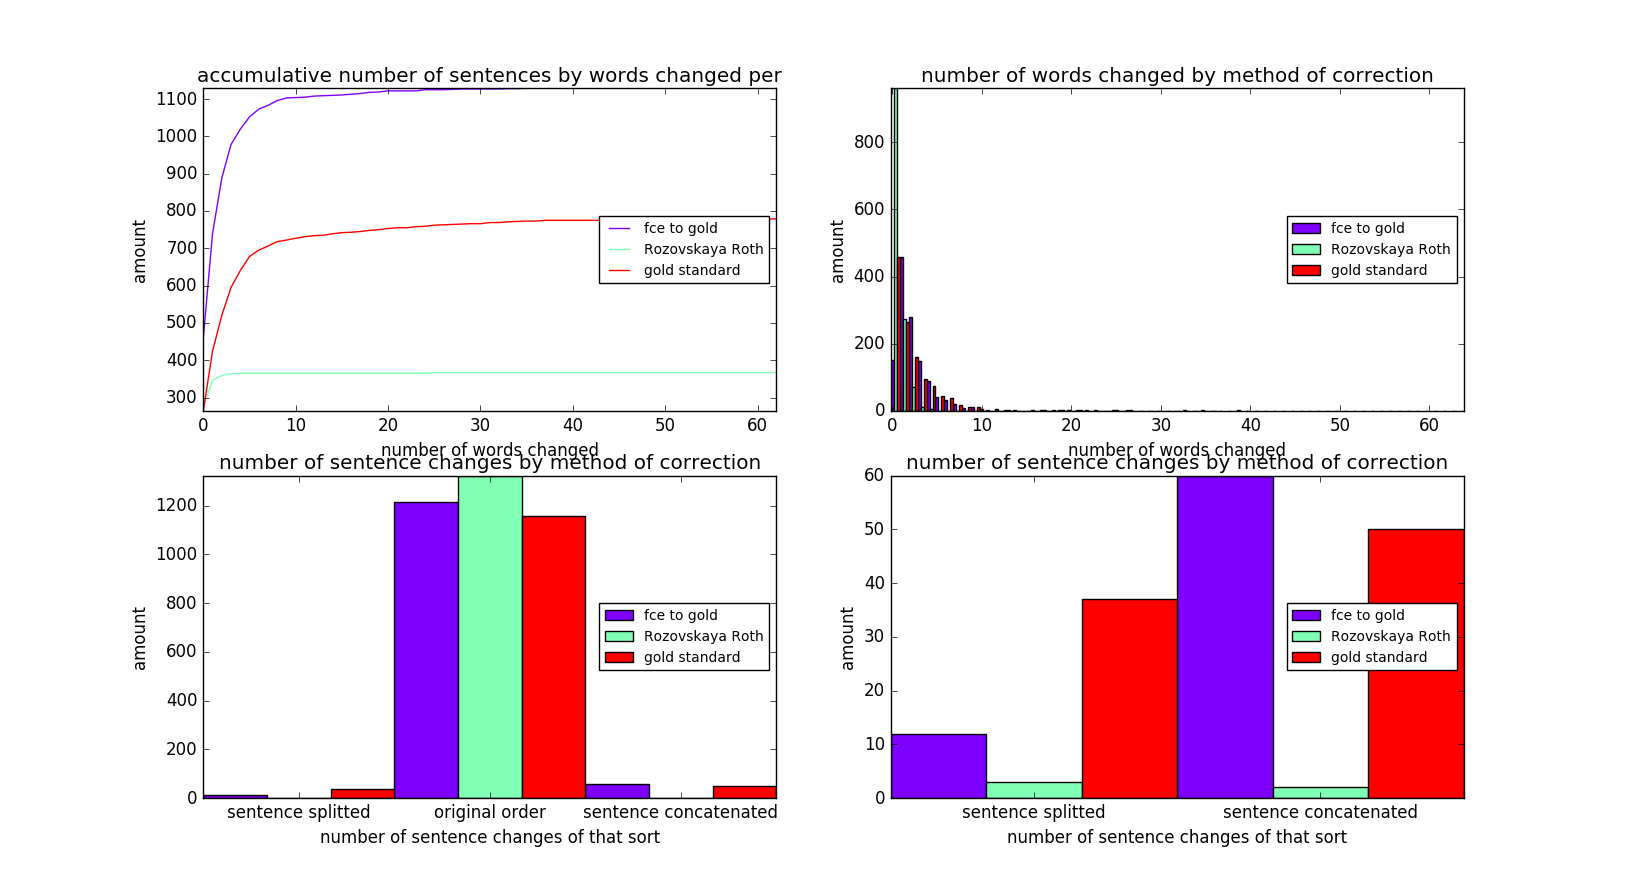
\includegraphics{figure_1}
	\caption{Sentences split and concatenated by different systems.}
	\label{fig:split}
\end{figure}

\begin{figure}
%	\includesvg{\detokenize{spearman_ecdftest.svg}}
	\caption{Spearman rho values by different systems.}
	\label{fig:rho}
\end{figure}

\begin{figure}
	\includesvg{alignedtest}
	\caption{Number of sentences with different number of words changed by different systems.}
	\label{fig:words_changed}
\end{figure}

\subsection{discussion}


Lets discuss the results in \ref{fig:words_changed}\ref{fig:rho} and \ref{fig:split} starting at what we see isn't change in the gold standard. We can think of it as what calls for formal conservatism. We see that it is most common for a sentence to have
no change, not to concatenate two consecutive sentences and not to
split a sentence into two. We also observe high correlation coefficient
for most of the sentences. Summing it all together we indeed have
more unchanged than changed in every measure we have. But, with a
closer look we should also notice that it mostly tells us about the
dataset. Specifically the level of English found in the dataset.
These measures should be seen as a gold standard of the amount of
corrections to be done, and as we might wish to be a bit conservative
and not exceed it, this is still where we should aim.

When we broaden our view and consider the results of the different
correctors, the picture is clear. All correctors are over conservative.
It is not only that correctors don't tend to overcorrect, they all,
to the last one, by all the measures we checked, undercorrect a lot
and are over conservative. A special case would be the cambridge output that has more sentences that have corrections than the gold standard, but unlike the gold standard almost all these sentences have 1 correction. {*}do the plots need textual analyzing? e.g. explain why do we see under correction in fig 1 2 3?{*}

%\begin{figure}
%\caption{\protect\includegraphics[width=8cm]{\string"graphs/formal conservatism/differences2_some_competitors\string".pdf}}
%text
%\end{figure}


\section{May lack of corrections lead to over formal conservatism?\label{sec:May-lack-of}}

\subsection{The idea}

Some corrections might really be too hard for current correctors to
correct, leading to cautious corrections. Another cause for over conservatism
might hide in the assessment methods. before we show it, lets assume
that each ungrammatical sentence has some possible corrections. From
the corrections only 2 are in the gold standard. That would lead to
problems in both assessment and development process. In the assessment,
results will not be reliable, having correct sentences regarded as mistakes. This leads to more fluctuations and low scores even for a perfect output.
Perhaps less obvious will be how it affects the development
process. Even if corrected well, sentences which have more possible
corrections will grant lower scores on precision for correcting, while recall will not grant high reward for correcting, as most of the time the correction will be considered false anyway. This, and especially in the precision oriented scenario, will lead, either through
machine learning or algorithm development cycles, to learn \textbf{not} to correct
those sentences at all. In the rest of this section we will show that the assumptions we made are the current reality. Additionally, we pursue a statistical investigation of correction distributions, assessment values and assessment significance.

\subsection{Corrections as a distribution}

Lets denote $X=x_{1}\ldots x_n\sim L$ as the considered
sentences for evaluation where $L$ is a distribution over all learner sentences from the domain . 
For each $D_{x_i}$ the distribution of corrections over a sentence $x_i$ there exists the set of gold standard annotations is $\left\{ y_{1}^{i},\ldots,y_{M}^{i}\right\} \sim D_{x_i}$. Currently, in all the common corpora $M$ is constant, we will treat it as such, but generalizing from $M$ in general to specific $m_i$ is trivial. The corrector's output is a function $f\left(x_{i}\right)$. A certain assessment statistic is a function $\hat{S}=Eval\left(f\left(x_{1}\right),\left\{ y_{1}^{1},\ldots,y_{M}^{1}\right\} \ldots,f\left(x_{N}\right),\left\{ y_{1}^{N},\ldots,y_{M}^{N}\right\} \right)$.

We found no work that describes or assesses the way $D_x$ distributions are, and we aim to do so now. 

\subsection{Our data}
To be able to answer interesting statistical questions about assessment we first need to understand the behaviour of the distributions $D_x$. For that we randomly picked 52 sentences with max length 15 from the Nus \cite{dahlmeier2013building} test data. The length condition was made to make crowdsourcing more reliable. It also made sure we will not capture many interleaving errors from text units that could have been separated. Also as manual analyzing suggested, very short sentences were regarded as sentence tokenization errors and discarded. Histogram of sentence lengths showed a lot of the mass is below this threshold.

Albeit too expensive for assessment of each development cycle, human assessment by crowdsourcing is a very useful tool. Crowdsourcing assessment was shown to be helpful in different tasks such as translation{*}cites -translation{*} and even more so in error correction\cite{madnani2011they}{*}are there more cites?{*} as error correction is a more intuitive task than translation. Thus, for each of the sentences gathered we asked Amazon Mechanical Turk workers to correct them, leading to 2600 corrections overall, 50 for every sentence. A couple of sentences did not need correction according to a large part of the workers and hence were discarded.

For each sentence we used UnseenEst \cite{zou2015quantifying}, a statistical algorithm that quantify the distribution of frequencies. Manual tests with different inputs were done with satisfying result. The distributions as quantified by UnseenEst have a large number of corrections with low probability and a rather small number of frequent corrections. For that reason, it might be reasonable to look at the distribution as taken from {*}power law? zipf? overall from a dirichlet process? we don't have anything more to say here?{*}, to account for the different hyperparameters and what determines them.

\subsection{Assessment values\label{sec:Assessment-values}}

The values an assessment process produces are the base foundation of
 every improvement in Computer Sciences. This gives the value an
  almost sacred place. We think this role should be earned and measured.
 
 We shall begin by analyzing accuracy. While this is not published it is the choice for training machine learning algorithms. We suggest its more common use for another important reason which is interpretability.
For simplicity we assume a system has a constant probability $c$ to correct an ungrammatical sentence. The probability to get a specific accuracy assessment over $N$ sentences will be distributed as $$\hat{S}\sim\frac{\sum_{i=1}^{N}Ber\left(c\cdot p_i\right)}{N} $$ 
where $p_i=p_{covered}\left(x_i\right) $ is the probability that the i'th sentence correction will be in the gold standard. 
$Ber\left(p\right)$ is a Bernoulli variable with probability $p$. This is a Poisson Binomial random variable divided by n. 

First, we are to look at some general properties.
 One interesting property is that the number of sentences considered does not change the expected accuracy value.
 Another property to consider is that the ratio between scores of different systems stays the same no matter what are $p_1,\ldots,p_n$. So in this assessment we get a reliable way of comparing two systems, but we underestimate performance depending on our coverage. The only way to get more coverage will be to acquire more annotations.
 
 \begin{figure}
 	%	\includesvg{exact__repeat_1000_accuracy.svg}
 	\caption{Mean accuracy values for perfect systems with different gold standard size.}
 	\label{fig:accuracy_vals}
 \end{figure}
 
Based on the corrections we gathered and the distribution estimation we numerically compute the average coverage of a given sentence given that we randomly sample $M$ corrections for our gold standard. For every $M$ we take the mean coverage of sentence $x_i$ to be $p_i$. This defines the Poisson binomial distributions. In \ref{fig:accuracy_vals} we show the expected accuracy of a randomly selected perfect system for different values of $M$. As mentioned earlier, this measure is the $100\%$ and the ratio for different $c$ values is the accuracy ratio between corresponding systems. This measures need not change when we enlarge the test data, the variance of the assessment is all that changes. So both when we consider the amount of annotations needed and a system performance, it would be advisable to take these numbers into account.

While accuracy is very popular for machine learning tasks, F score is currently the only measure to be published in articles. As F score is much more complicated, no analytical way to predict its value was proposed \cite{yeh2000more}. 

We assess different expected results for perfect outputs with different $M$ values (see \ref{fig:F_Ms}). It is a challenge to do that without generating a whole dataset with enough annotations plus a large test set to account for the variability of different annotators. We sample for each ungrammatical sentence in the gold standard a sentence from our data set and $M$ corrections uniformly sampled from the empirical distribution we have collected. We also sample a perfect output in the same way (with $M=1$). With that we use the many corrections for each sentence to account for annotation variability and hold the ratios of different corrections stable. At last, we transform each of the corrections into a set of edits as requested by the $M^2$ scorer\cite{dahlmeier2012better}.  

This would be a good place to mention the drawbacks and assumptions of the methods we are using. We assume that the sentences we picked are a good representation of the overall sentences, but know they might be a bit simpler as we did not choose very large sentence for the reasons mentioned earlier. Another assumption which puts the way assessment is done under the spotlight is that our machine based edits are good enough for assessment. Edits do not only add variability that it is hard to account for, they are also much harder to get agreement on. 

To conclude, on both measures we see a large improvement in coverage when enlarging $M$ suggesting that a more reasonable $M$ to choose would be somewhere around 8 where the high probability corrections are probably covered and the graph turns semi-linear. The results also strongly support the hypothesis assessment values are very low, and hence might be a cause for over conservatism.
 Another conclusion to be made is that given a value from the assessment process we may estimate how low the value is in respect to the perfect assessment. Some may wish to correct for this under assessment.

\section{On significance and variation}

So far we have discussed the mean values of the assessment and showed they are lower bounds of the real values of the same assessment with a full gold standard. For some uses the value itself does not matter, what really matters is whether one value is significantly higher than another value. The assumption about significance was that with enough sentences this problem can be overcome.

We wish to show a somewhat more complex point of view, stating that the way to reduce variation in assessment values would be to balance between the number of sentences and the number of annotations per sentence. We also provide the numbers needed for choosing how to balance wisely. 

Choosing how to balance is dependent on the goals of the one collecting data, and affects the mean value as well, as discussed in \ref{sec:Assessment-values}. Thus, we will not discuss this issue here and just point out that such questions have been studied in various fields such as genetics\cite{ionita2010optimal}.

So, why is significance more complicated? Basically, because variance is more complex than mean. While $\mathbb{E}_{y\sim d_x, x\sim L}\left(\hat{S}\right)$ vary only as we change $M$
the number of annotations, but not $N$ the number of corrections,
$Var_{y\sim d_x, x\sim L}(\hat{S})$ depends on both. We try to assess and give an upper
bound on how much it varies for different $M$ and $N$, allowing
for both a smart allocation of resources when building a corpus and
for assessing on given corpora whether two systems are actually different.

\subsection{Significance}

\begin{figure}
	%	\includesvg{exact__repeat_1000_accuracy.svg}
	\caption{F Score results with different sizes of gold standard.}
	\label{fig:F_Ms}
\end{figure}
\begin{figure}
	%	\includesvg{exact__repeat_1000_accuracy.svg}
	\caption{F Score results for different systems including confidence interval.}
	\label{fig:F_systems}
\end{figure}


As before, we start considering the analytic formalism we have for accuracy. For that, sentences which were not corrected, or wrongly corrected have no variance with different $m$s, corrected sentences do. The variation of the Poisson binomial random variable we have is $\sum_{i=1}^{n}p_i\cdot\left(1-p_i\right)$ and as we divide the variable by $n$ we get $\frac{\sum_{i=1}^{n}p_i\cdot\left(1-p_i\right)}{n^2}$. 
The variation is proportional to the square of the number of sentences chosen given fixed $p_i$ values. Given a fixed $N$ variation gets lower as $p_i$s get away from $0.5$, a change that, from a certain point, occurs when $M$ is increased.

We use bias-corrected and accelerated bootstrap \cite{efron1987better}, to assess the $95\%$ confidence interval of different systems with the current NUS test data ($m=2$), based on the same process as in \ref{sec:Assessment-values}. Results can be seen in \ref{fig:F_systems}.

\subsection{discussion}

If the NLP community has agreed one correction is not enough\cite{tetreault2008native}
we can now say 2 is no magic number either. We can also see the effect of different references amounts on significance and actual value of both accuracy and precision, recall and F score.
We see that considering the changed indexes, looking for example at different synonyms as the same correction, still holds a very large number of different corrections for every sentence.


\bibliographystyle{acl_natbib}
\bibliography{propose}

\section{Appendix}

\end{document}
